\section{Electric Connector Plug Insertion Tasks}

In this work, we empirically evaluate learning methods on a set of electric connector assembly tasks, pictured in Fig.~\ref{fig:usb_photo_demo2}.
Connector plug insertions are difficult for two reasons. 
First, the robot must be very precise in lining up the plug with its socket. 
\begin{wrapfigure}[14]{r}{0.5\textwidth}
  \begin{center}
    %\vspace{12pt}
        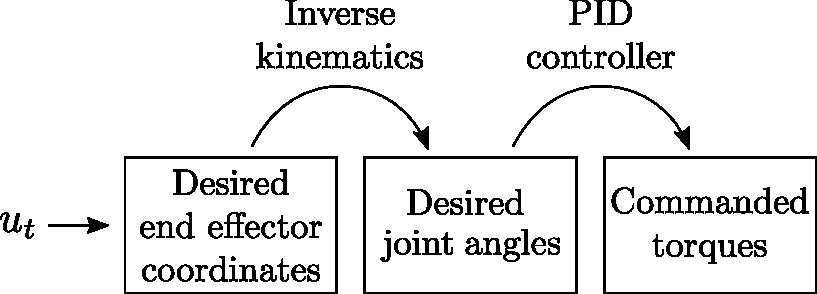
\includegraphics[width=0.88\linewidth]{insertion/newfigs/control_pipeline.pdf}
        %\vspace{6pt}
        \captionsetup{justification=justified, format=plain}
    \caption{Illustration of the robot's cascade control scheme. The actions  $u_t$ are computed at a frequency of up to $10\,\mathrm{Hz}$,  desired joint angles are obtained by inverse kinematics, and a joint-space impedance controller with anti-windup PID control commands actuator torques at $1000\,\mathrm{Hz}$.}
   \label{fig:control_pipeline}
  \end{center}
\end{wrapfigure}
As we show in our experiments, errors as small as~$\pm 1$\,mm can lead to consistent failure. 

Second, there is significant friction when the connector plug touches the socket, and the robot must learn to apply sufficient force in order to insert the plug. Image sequences of successful insertions are shown in Fig.~\ref{fig:usb_photo_demo2}, where it is also possible to see details of the gripper setup that we used to ensure a failure free, fully automated training process.
In our experiments, we use a 7 degrees of freedom Sawyer robot with end-effector control, meaning that the action signal $u_t$ can be interpreted as the relative end-effector movement in Cartesian coordinates. The robot's underlying internal control pipeline is illustrated in Figure~\ref{fig:control_pipeline}.

To comprehensively evaluate connector assembly tasks, we experiment on a variety of connectors. Each connector offers a different challenge in terms of required precision and force to overcome friction. 
We chose to benchmark the controllers performance on the insertion of a USB connector, a U-Sub connector, and a waterproof Model-E connector manufactured by MISUMI.
All the explored use cases were part of the IROS 2017 Robotic Grasping and Manipulation Competition \cite{roboticgrasping2017iros}, included as part of a task board developed by NIST to benchmark the performance of assembly robots.

\subsection{Adapters}
In the following we describe the used adapters, USB, D-Sub, and Model-E. The observed difficulty of the insertion increases in that order.

\textbf{USB.} The USB connector is a ubiquitous, widely-used connector and offers a challenging insertion task. Because the adapter becomes smoother and therefore easier to insert over time due to wear and tear, we periodically replace the adapter. Of the three tested adapters, the USB adapter is the easiest.

\textbf{D-sub.} Inserting this adapter requires aligning several pins correctly, and is therefore more sensitive than inserting the USB adapter. It also requires more downward force due to a tighter fit.

\textbf{Model-E.} This adapter is the most difficult of the three tested connectors as it contains several edges and grooves to align and requires significant downward force to successfully insert the part.

\subsection{Experimental Settings}
We consider three settings in our experiments in order to evaluate how plausible it is to solve these tasks with more convenient state representations and reward functions and to evaluate the performance of different algorithms changes as the setting is modified.

% \subsubsection{Visual}
\textbf{3.2.1 Visual. } In this experiment, we evaluate whether the RL algorithms can learn to perform the connector assembly tasks from vision without having access to state information. The state provided to the learned policy is a $32 \times 32$ grayscale image, such as shown in Fig.~\ref{fig:vision_insertion_sequence}.

\vspace{1cm}
\begin{wrapfigure}{r}{0.5\textwidth}
% \begin{figure}[t]
\centering
\resizebox{.95\linewidth}{!}{
    \begin{subfigure}[b]{0.24\linewidth}
        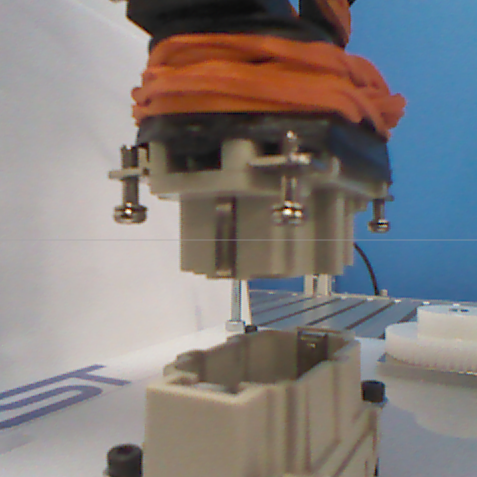
\includegraphics[width=0.99\linewidth]{insertion/robot_view_screenshots/waterproof_s2_square.png}\\
        \centering
    \end{subfigure}
    \begin{subfigure}[b]{0.24\linewidth}
        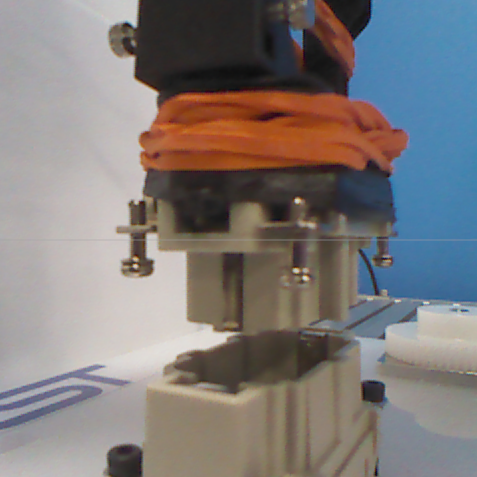
\includegraphics[width=0.99\linewidth]{insertion/robot_view_screenshots/waterproof_s3_square_.png}\\
        \centering
    \end{subfigure}  
    \begin{subfigure}[b]{0.24\linewidth}
        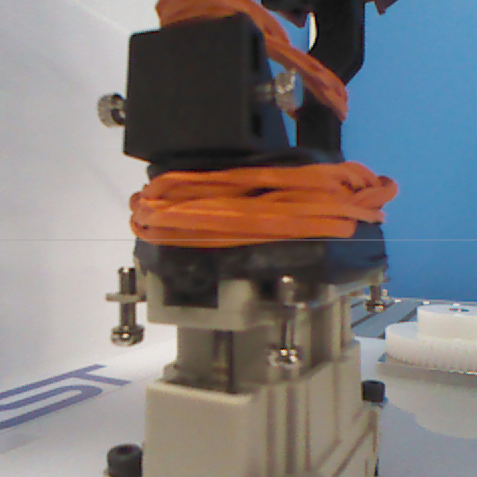
\includegraphics[width=0.99\linewidth]{insertion/robot_view_screenshots/waterproof_s4_square.png}\\
        \centering
    \end{subfigure} 
    \begin{subfigure}[b]{0.24\linewidth}
        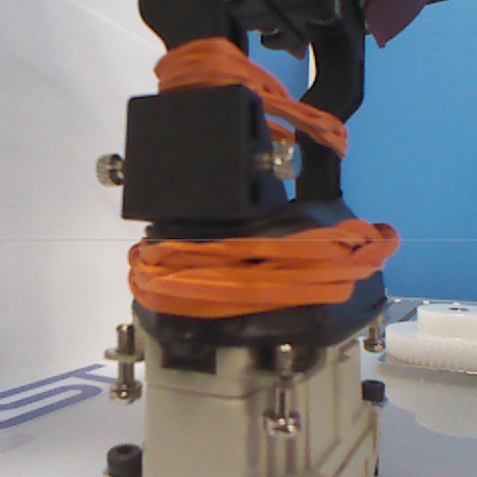
\includegraphics[width=0.99\linewidth]{insertion/robot_view_screenshots/waterproof_s7_square.png}\\
        \centering
    \end{subfigure}
    }
    \\
    \vspace{-6pt}
    \resizebox{.95\linewidth}{!}{
    \begin{subfigure}[b]{0.24\linewidth}
        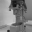
\includegraphics[width=0.99\linewidth]{insertion/robot_view_screenshots/water_target_image2.png}\\
        \centering
    \end{subfigure} 
    \begin{subfigure}[b]{0.24\linewidth}
        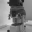
\includegraphics[width=0.99\linewidth]{insertion/robot_view_screenshots/water_target_image3.png}\\
        \centering
    \end{subfigure}     
    \begin{subfigure}[b]{0.24\linewidth}
        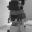
\includegraphics[width=0.99\linewidth]{insertion/robot_view_screenshots/water_target_image4.png}\\
        \centering
    \end{subfigure} 
    \begin{subfigure}[b]{0.24\linewidth}
        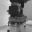
\includegraphics[width=0.99\linewidth]{insertion/robot_view_screenshots/water_target_image1.png}\\
        \centering
    \end{subfigure}   
     }
     \captionsetup{justification=justified, format=plain}
    \caption{Successful insertion on the Model-E connector. The image-based RL algorithms receives only receives the $32\times32$ grayscale image as the observation.
    % is the only observation that the image-based RL algorithm receives.
    }
    %\vspace{9pt}
    \label{fig:vision_insertion_sequence}
% \end{figure}
\end{wrapfigure}
For goal specification, we use a goal image, avoiding the need for state information to compute rewards. The reward is the pixelwise L1 distance to the given goal image. Being able to learn from such a setup is compelling as it does not require any extra state estimation and many tasks can be specified easily by a goal image.

\textbf{3.2.2. Sparse. } In this experiment, the reward is obtained by directly measuring whether the connection is alive and transmitting:

\vspace*{0cm}
\begin{align}
 r  = 
  \begin{cases}
    1, & \text{if insertion signal detected } \\
    0, & \text{else. } \\
  \end{cases}
\end{align}
This is the exact true reward for the task of connecting a cable, and can be naturally obtained in many manufacturing systems. As state, the robot is given the Cartesian coordinates of the end-effector $x_t$ and the vertical force $f_z$ that is acting on the end-effector. We could only automatically detect the USB connection, so we only include the USB adapter for the sparse experiments. 

\textbf{3.2.3. Dense. } In this experiment, the robot receives a manually shaped reward based on the distance to the target location $ x^{*}$. We use the reward function
\begin{equation}
r_t =  - \alpha \cdot {\Vert x_t - x^{*} \Vert}_1 -  \frac{\beta}{\left({\Vert x_t - x^{*} \Vert}_2 + \varepsilon\right)} - \varphi \cdot f_z,
\label{eq:shaped_reward_function}
\end{equation}
where $0 < \varepsilon \ll 1$. 
The hyperparameters are set to ${\alpha = 100}$, ${\beta = 0.002}$, and ${\varphi = 0.1}$. When an insertion is indicated through a distance measurement, the sign of the force term flips, so that $\varphi = -0.1$ when the connector is inserted. This rewards the agent for pressing down after an insertion and showed to improve the learning process.
The force measurements are calibrated before each rollout to account for measurement bias and to decouple the measurements from the robot pose. 
